\documentclass[10pt]{beamer}

\usepackage[T1]{fontenc}
\usepackage[utf8]{inputenc}
\usepackage{microtype}
\usepackage{amsmath}
\usepackage{amssymb}
\usepackage{graphicx}
\usepackage{booktabs}
\usepackage{natbib}
\usepackage[dvipsnames]{xcolor}

% \usepackage[hypertexnames=false,hidelinks]{hyperref}
% \usepackage[noabbrev,nameinlink,capitalize]{cleveref}

\bibliographystyle{agsm}

\newcommand{\Parametric}{\textbf{\textcolor{ForestGreen}{Parametric}}}
\newcommand{\Contextual}{\textbf{\textcolor{Maroon}{Contextual}}}
\newcommand{\Other}{\textbf{\textcolor{MidnightBlue}{Other}}}

\graphicspath{{.}{./pictures}{./figures}}

\title{Knowledge Grounding in Language Models: An Empirical Study}
\author{Martin Fixman}
\date{UCL Medical Physics and Biomedical Engineering \\[2mm] 10-Minute PhD Presentation}

\begin{document}

\begin{frame}
Introduction.

Large Language Models (LLMs) offer state-of-the-art performance on many tasks.
However, hallucinations remain problematic in mission-critical contexts.

\end{frame}

\begin{frame}{Motivation and Research Question}
Motivation.

Retrieval-Augmented Generation (RAG) is a promising way to mitigate hallucinations by providing external context to an LLM.

Research Question.

How do LLMs respond if the context provided contradicts what they have memorized in their parameters?

\end{frame}

\begin{frame}{Method: Framework Overview}
Here is an overview of the experimental setup.

\begin{itemize}
  \item Generate a diverse dataset of short-answer questions.
  \item Query the model without extra context to get a \Parametric{} answer.
  \item Add a \emph{counterparametric} context that contradicts the original model answer.
  \item Re-query with the new contradictory context.
  \item Compare the new response against parametric vs.\ contextual data.
\end{itemize}

\begin{center}
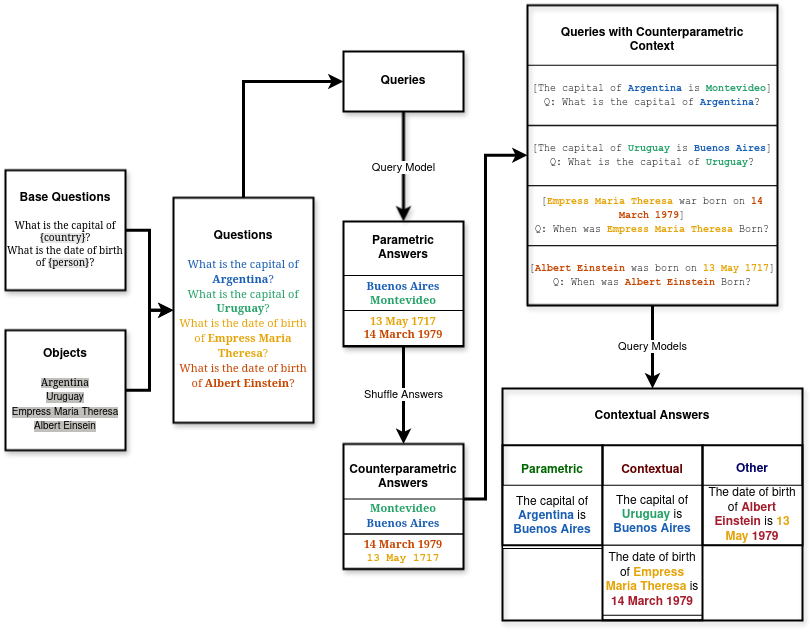
\includegraphics[width=0.7\textwidth]{Method.png}
\end{center}

\end{frame}

\begin{frame}{Results: Parametric vs.\ Contextual}
We tested four models: two Seq2Seq (Flan-T5) and two Decoder-only (Llama).

\begin{itemize}
  \item \Contextual{} answers dominate in Seq2Seq models.
  \item Decoder-only models more often ignore contradictory context and revert to \Parametric{} knowledge.
\end{itemize}

\begin{center}
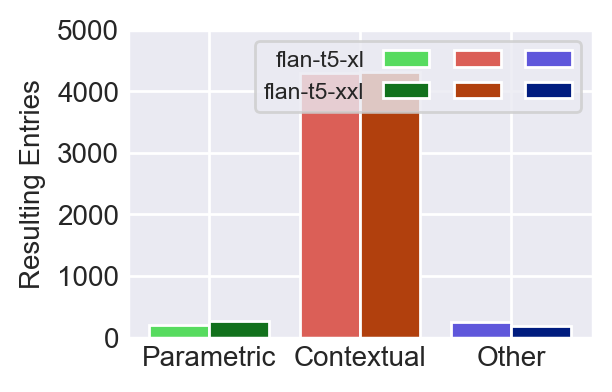
\includegraphics[width=0.66\textwidth]{flan_amount.png}
\end{center}

\end{frame}

\begin{frame}{Discussion: Model Architecture and Size}
Seq2Seq models (encoder-decoder) appear more sensitive to external context.

\begin{itemize}
  \item \textbf{Flan-T5-XL and Flan-T5-XXL}: minimal difference in using context despite large size gap.
  \item \textbf{Llama-8B vs.\ Llama-70B}: bigger model reverts to parametric memory more often.
\end{itemize}

Conclusion.

Bigger Decoder-only models are more likely to trust memorized facts over a contradictory context, while Seq2Seq architectures generally rely on provided context.

\end{frame}

\begin{frame}{Future Work}
Refine string-comparison to handle partial rephrasings.

Extend experiments to:
\begin{itemize}
  \item RAG-specific models like \textsc{Atlas} or \textsc{Retro}.
  \item Fine-tuning large language models to better trust contradictory context.
  \item Using perplexity signals to detect hallucinations and selectively re-query the retriever.
\end{itemize}

\end{frame}

\begin{frame}{References}
\small

\bibliography{knowledge_grounding}

\end{frame}

\begin{frame}
\centering
\Large
Thank you. Questions?
\end{frame}

\end{document}

